\documentclass[12pt]{article}

% Packages
\usepackage[utf8]{inputenc}
\usepackage{amsmath, amssymb}
\usepackage{graphicx}
\usepackage{fancyhdr}
\usepackage{geometry}
\usepackage{algorithm}
\usepackage{algpseudocode}
\usepackage{caption}
\geometry{margin=1in}

% Header/Footer Configuration
\pagestyle{fancy}
\fancyhf{}
\fancyhead[L]{\yourname}
\fancyhead[C]{Homework \#6}
\fancyhead[R]{\coursecode}
\fancyfoot[C]{\thepage}

% Custom commands
\newcommand{\yourname}{Surabhi Raghavan}  % Your name
\newcommand{\hwnumber}{6}          % Homework number
\newcommand{\coursecode}{INFSCI 2591}  % Course name/code

% Begin document
\begin{document}

\title{Homework \#6}
\author{\yourname}
\date{\today}

\maketitle

\section*{Problem 4}
% Problem description
Write an algorithm that takes an integer n as input and determines the total
number of solutions to the n-Queens problem.
\subsection*{Solution}
% Your solution goes here.
The n-queens problem  involves placing n queens on a n x n chessboard such that no two queens threaten each other.
\\
Two queens do not threaten each other if:
\begin{itemize}
\item if 2 queens are in the same row
\item if 2 queens are in the same column 
\item if 2 queens are iin the same diagonal 
\end{itemize}
We need two separate functions- one to place the queen in a particular position and another to determine all combinations of the solutions.\\
\\
Alogrithm: Determine if a queen can  be placed at a particular position \\
Input: k (int)- represents the kth queen \\
Output: Returns 1 if the queen can be placed and 0 if it cannot\\

\begin{algorithm}
    \caption{Place($k, i$)}
    \begin{algorithmic}[1]
        \For{$j = 1$ to $k-1$}
            \If{$x[j] = i$ \textbf{or} $|j - k| = |x[j] - i|$}
                \State \Return 0
            \EndIf
        \EndFor
        \State \Return 1
    \end{algorithmic}
    \end{algorithm}
    

Alogrithm: Function to determine the number of solutions to the n-queens problem\\
Input: n (int)- represents the number of queens and the size of the chessboard \\
Output: Number of solutions\\

\begin{algorithm}
    \caption{NQueens(n)}
    \begin{algorithmic}[1]
        \State $k \gets 1$
        \State $x[k] \gets 0$
        \State $solution\_count \gets 0$ \Comment{Initialize counter for number of solutions}
        \While{$k > 0$}
            \State $x[k] \gets x[k] + 1$
            \While{$x[k] \leq n$ \textbf{and} not PLACE($k, x[k]$)}
                \State $x[k] \gets x[k] + 1$
            \EndWhile
            \If{$x[k] \leq n$}
                \If{$k == n$}
                    \State $solution\_count \gets solution\_count + 1$ \Comment{Increment solution count}
                \Else
                    \State $k \gets k + 1$
                    \State $x[k] \gets 0$
                \EndIf
            \Else
                \State $k \gets k - 1$
            \EndIf
        \EndWhile
        \State \Return $solution\_count$ \Comment{Return the total number of solutions found}
    \end{algorithmic}
    \end{algorithm}
\section*{Problem 10}
% Problem description
Find at least two instances of the n-Queens problem that have no solutions.
\subsection*{Solution}
There are 2 cases in which the n-Queens problem has no solutions.\\
I figured it out by manually placing queens on the chessboard. It was quickly determined that there was no position where the queens didn't threaten each other.\\

\textbf{CASE 1: No Solution for $n = 2$} \\[12pt]

Consider a 2 x 2 chessboard. When $n = 2$, we need to place 2 queens on the chessboard, with each queen occupying its own row and column. We start by placing the first queen at position a2 (as shown in Fig. 1). Now, we need to place the second queen in one of the remaining three positions. However, no matter where we place the second queen, it will either be in the same row, the same column, or the same diagonal as the first queen.

\begin{itemize}
    \item The queen cannot be placed at b2, as it would be in the same row as the first queen (Fig. 2).
    \item The queen cannot be placed at a1, as it would be in the same column as the first queen (Fig. 3).
    \item The queen cannot be placed at b1, as it would be in the same diagonal as the first queen (Fig. 4).
\end{itemize}

Thus, there is no valid way to place two queens on a 2x2 chessboard without them threatening each other.

% Creating a figure environment for better control over positioning of images
\begin{figure}[h]
    \centering
    \begin{minipage}{0.2\textwidth}
        \centering
        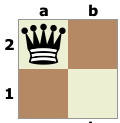
\includegraphics[width=\textwidth]{Fig1.png}
        \captionof{figure}{Initial Positioning of the Queen (a2)}
    \end{minipage}
    \hspace{0.05\textwidth} % Horizontal space between images
    \begin{minipage}{0.2\textwidth}
        \centering
        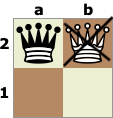
\includegraphics[width=\textwidth]{Fig2.png}
        \captionof{figure}{Queen cannot be placed in the same row (b2)}
    \end{minipage}
    
    \vspace{0.5cm} % Vertical space between rows of images
    
    \begin{minipage}{0.2\textwidth}
        \centering
        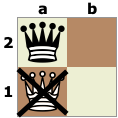
\includegraphics[width=\textwidth]{Fig3.png}
        \captionof{figure}{Queen cannot be placed in the same column (a1)}
    \end{minipage}
    \hspace{0.05\textwidth} % Horizontal space between images
    \begin{minipage}{0.2\textwidth}
        \centering
        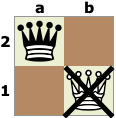
\includegraphics[width=\textwidth]{Fig4.png}
        \captionof{figure}{Queen cannot be placed on the diagonal (b1)}
    \end{minipage}
\end{figure}



\textbf{CASE 2: No Solution for $n = 3$} \\[12pt]

Consider a 3 x 3 chessboard. When $n = 3$, we need to place 3 queens on the chessboard, with each queen occupying its own row and column. We start by placing the first queen at position a3 (as shown in Fig. 1). Now, we need to place the second queen in one of the remaining three positions. However, no matter where we place the second queen, it will either be in the same row, the same column, or the same diagonal as the first queen.

\begin{itemize}
    \item The queen cannot be placed at b3 or c3, as it would be in the same row as the first queen (Fig. 6).
    \item The queen cannot be placed at a2 or a1, as it would be in the same column as the first queen (Fig. 7).
    \item The queen cannot be placed at b2 or c1, as it would be in the same diagonal as the first queen (Fig. 8).
\end{itemize}

The only positions remaining are c2 or b1. We can place the second queen in either of these positions. I will choose to place it at c2 (Fig. 9). Fig 10: Shows us that there is no other position to place the third queen. 
The same would be shown for any other position of the queens. 

% Creating a figure environment with 3 images per row
\begin{figure}[h]
    \centering
    % First row of 3 images
    \begin{minipage}{0.3\textwidth}
        \centering
        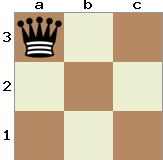
\includegraphics[width=\textwidth]{Fig5.png}
        \captionof{figure}{Queen at a3}
    \end{minipage}
    \hspace{0.03\textwidth}
    \begin{minipage}{0.3\textwidth}
        \centering
        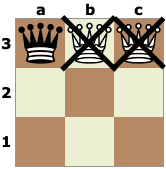
\includegraphics[width=\textwidth]{Fig6.png}
        \captionof{figure}{Cannot be placed in the same row (b3, c3)}
    \end{minipage}
    \hspace{0.03\textwidth}
    \begin{minipage}{0.3\textwidth}
        \centering
        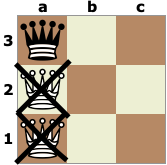
\includegraphics[width=\textwidth]{Fig7.png}
        \captionof{figure}{Cannot be placed in the same column (a2, a1)}
    \end{minipage}

    \vspace{0.5cm} % Vertical space between rows
    
    % Second row of 3 images
    \begin{minipage}{0.3\textwidth}
        \centering
        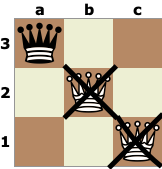
\includegraphics[width=\textwidth]{Fig8.png}
        \captionof{figure}{Cannot be placed on the diagonal (b2, c1)}
    \end{minipage}
    \hspace{0.03\textwidth}
    \begin{minipage}{0.3\textwidth}
        \centering
        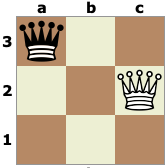
\includegraphics[width=\textwidth]{Fig9.png}
        \captionof{figure}{Second queen placed at c2}
    \end{minipage}
    \hspace{0.03\textwidth}
    \begin{minipage}{0.3\textwidth}
        \centering
        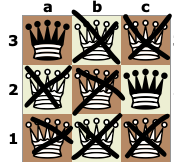
\includegraphics[width=\textwidth]{Fig10.png}
        \captionof{figure}{Third queen scenario- cannot be placed anywhere}
    \end{minipage}
\end{figure}

\section*{Problem 13}
% Problem description
Use the Backtracking algorithm for the Sum-of-Subsets problem (Algorithm 5.4) to find all combinations of the following numbers that sum to \( W = 52 \):

\[
w_1 = 2, \quad w_2 = 10, \quad w_3 = 13, \quad w_4 = 17, \quad w_5 = 22, \quad w_6 = 42
\]
Show the actions step by step.
\subsection*{Solution}
% Your solution goes here.
\begin{algorithm}
    \caption{sum\_of\_subsets(index $i$, int weight, int total)}
    \begin{algorithmic}[1]
        \If{promising($i$)}
            \If{weight $=$ $W$}
                \State \textbf{Output:} subset from $include[1]$ through $include[i]$
            \Else
                \State include[$i+1$] $=$ "yes"
                \State sum\_of\_subsets($i+1$, weight + $w[i+1]$, total - $w[i+1]$) \Comment{Include $w[i+1]$}
                
                \State include[$i+1$] $=$ "no"
                \State sum\_of\_subsets($i+1$, weight, total - $w[i+1]$) \Comment{Do not include $w[i+1]$}
            \EndIf
        \EndIf
    \end{algorithmic}
\end{algorithm}

Promising Function

\begin{algorithm}
    \caption{promising(index $i$)}
    \begin{algorithmic}[1]
        \State \textbf{Return:} $(weight + total \geq W)$ \textbf{and} $(weight + w[i+1] \leq W)$
    \end{algorithmic}
\end{algorithm}
\end{document}
